\chapter{Game AI}
\label{apdx:gameAI}

\section{Negamax}

\begin{algorithm}
\caption{Negamax algorithm (with closures)}
\label{alg:negamax}
\begin{algorithmic}
\Function{negamax}{depth}
    \If{$depth \leq 0$}
        \State \Return $value()$
    \EndIf
    \State $\alpha \leftarrow -\infty$
    \ForAll{possible moves}
        \State $\alpha \leftarrow max(\alpha, -negamax(depth-1))$
    \EndFor
    \State \Return $\alpha$
\EndFunction
\end{algorithmic}
\end{algorithm}

%%% function MonteCarloPlanning(state)
%%% 2: repeat
%%% 3: search(state, 0)
%%% 4: until Timeout
%%% 5: return bestAction(state,0)
%%% 6: function search(state, depth)
%%% 7: if Terminal(state) then return 0
%%% 8: if Leaf(state; d) then return Evaluate(state)
%%% 9: action := selectAction(state, depth)
%%% 10: (nextstate; reward) := simulateAction(state, action)
%%% 11: q := reward + ° search(nextstate, depth + 1)
%%% 12: UpdateValue(state; action; q; depth)
%%% 13: return q

\section{``Gamers' survey'' in section~\ref{surveygamers} page~\pageref{surveygamers}}

\label{apdx:survey}
\subsubsection{Questions}

How good are you?
\begin{itemize}
    \item Very good
    \item Good
\end{itemize}


How important is the virtuosity? (to win the game)
reflexes, accuracy, speed, "mechanics"
\begin{itemize}
    \item 0 (not at all, or irrelevant)
    \item 1 (counts, can be game changing for people on equal level at other answers)
    \item 2 (counts a lot, can make a player win even if he is a little worse on lower importance gameplay features)
\end{itemize}


How important is deductive thinking? (to win the game)
"If I do A he can do B but not C" or "I see E so he has done D", also called analysis, forward inference."
\begin{itemize}
    \item 0 (not at all, or irrelevant)
    \item 1 (counts, can be game changing for people on equal level at other answers)
    \item 2 (counts a lot, can make a player win even if he is a little worse on lower importance gameplay features)
\end{itemize}


How important is inductive thinking? (to win the game)
"He does A so he may be thinking B" or "I see D and E so (in general) he should be going for F (learned)", also called generalization, "abstraction".
\begin{itemize}
    \item 0 (not at all, or irrelevant)
    \item 1 (counts, can be game changing for people on equal level at other answers)
    \item 2 (counts a lot, can make a player win even if he is a little worse on lower importance gameplay features)
\end{itemize}


How hard is decision-making? (to win the game)
"I have options A, B and C, with regard to everything I know about this game, I will play B (to win)", selection of a course of actions.
\begin{itemize}
    \item 0 (not at all, or irrelevant)
    \item 1 (counts, can be game changing for people on equal level at other answers)
    \item 2 (counts a lot, can make a player win even if he is a little worse on lower importance gameplay features)
\end{itemize}


You can predict the next move of your opponent:
(is knowledge of the game or of the opponent more important)
\begin{itemize}
    \item 1 by knowing what the best moves are / the best play for him?
    \item -1 by knowing him personally (psychology)?
    \item 0 both equal
\end{itemize}


What is more important:
\begin{itemize}
    \item 1 knowledge of the game (general strategies, tactics, timings)
    \item -1 knowledge of the map (specific strategies, tactics, timings)
    \item 0 both equal
\end{itemize}

\subsubsection{Results}

\begin{sidewaystable}

\begin{tabular}{|l|ccc|ccc|ccc|ccc|ccc|ccc|}
\hline
Game & \multicolumn{3}{|c|}{Virtuosity} & \multicolumn{3}{|c|}{Deduction} & \multicolumn{3}{|c|}{Induction} & \multicolumn{3}{|c|}{Decision-Making} & \multicolumn{3}{|c|}{Opponent} & \multicolumn{3}{|c|}{Knowledge}\\
 & \multicolumn{3}{|c|}{(sensory-motor)} & \multicolumn{3}{|c|}{(analysis)} & \multicolumn{3}{|c|}{(abstraction)} & \multicolumn{3}{|c|}{(acting)} & \multicolumn{3}{|c|}{-1: subjectivity} & \multicolumn{3}{|c|}{-1: map} \\
 & \multicolumn{3}{|c|}{[0-2]} & \multicolumn{3}{|c|}{[0-2]} & \multicolumn{3}{|c|}{[0-2]} & \multicolumn{3}{|c|}{[0-2]} & \multicolumn{3}{|c|}{1: objectivity} & \multicolumn{3}{|c|}{1: game} \\
 & top & rest & n & top & rest & n & top & rest & n & top & rest & n & top & rest & n & top & rest & n \\
\hline
Chess &  X & X & X  & 1.714 & 1.815 & 34 & 1.714 & 1.429 & 35 & 1.714 & 1.643 & 35 & 0.714 & 0.286 & 35 &  X & X & X  \\
Go &  X & X & X  & 2.000 & 1.667 & 16 & 2.000 & 1.600 & 16 & 2.000 & 1.600 & 16 & 1.000 & 0.533 & 16 &  X & X & X  \\
Poker &  X & X & X  & 1.667 & 0.938 & 22 & 1.667 & 1.562 & 22 & 1.333 & 1.625 & 22 & -0.167 & -0.375 & 22 &  X & X & X  \\
Racing & 2.000 & 1.750 & 19 & 0.286 & 0.250 & 19 & 0.571 & 0.000 & 19 & 1.286 & 0.833 & 19 & 0.571 & 0.455 & 18 & -0.286 & -0.333 & 19 \\
TeamFPS & 1.917 & 1.607 & 40 & 1.083 & 1.000 & 39 & 1.417 & 0.929 & 40 & 1.417 & 1.185 & 39 & 0.000 & 0.214 & 40 & -0.083 & -0.115 & 38 \\
FFPS & 2.000 & 2.000 & 22 & 1.250 & 1.000 & 21 & 1.125 & 1.077 & 21 & 1.125 & 1.231 & 21 & 0.250 & -0.154 & 21 & 0.250 & 0.083 & 20 \\
MMORPG & 1.118 & 1.000 & 29 & 1.235 & 0.833 & 29 & 1.176 & 1.000 & 29 & 1.235 & 1.250 & 29 & 0.471 & 0.250 & 29 & 0.706 & 0.833 & 29 \\
RTS & 1.941 & 1.692 & 86 & 1.912 & 1.808 & 86 & 1.706 & 1.673 & 83 & 1.882 & 1.769 & 86 & 0.118 & 0.288 & 86 & 0.412 & 0.481 & 86 \\
\hline
\end{tabular}
\label{fullsurveygamers}
\caption{Results of the survey (means) for ``top'' players and the ``rest'' of answers, along with the total number of answers (n).}
\end{sidewaystable}

%\chapter{Strategy}
%
%\section{Openings }
%NED stands for Not Enough Data\\
%Win rates of columns vs lines\\
%
%\begin{tabular}{|l|cccccc|}
%\hline
% & two gates & fast dt & speedzeal & reaver drop & corsair & nony\\
%\hline
%two gates &  0.5 & NED & NED & NED & NED & NED \\
%fast dt &  NED & 0.5 & NED & 0.454545454545 & NED & 0.445544554455 \\
%speedzeal &  NED & NED & NED & NED & NED & NED \\
%reaver drop &  NED & 0.545454545455 & NED & NED & NED & 0.608695652174 \\
%corsair &  NED & NED & NED & NED & NED & NED \\
%nony &  NED & 0.554455445545 & NED & 0.391304347826 & NED & 0.5 \\
%\hline
%\end{tabular}
%PvP Total Games: 296

%%% \begin{tabular}{|l|cccccc|}
%%% \hline
%%%  & two gates & fast dt & unknown & reaver drop & corsair & nony\\
%%% \hline
%%% bio &  NED & NED & NED & NED & NED & NED \\
%%% unknown &  NED & NED & 0.5 & NED & NED & NED \\
%%% drop &  NED & NED & NED & NED & NED & NED \\
%%% two facto &  NED & 0.552083333333 & NED & 0.477272727273 & NED & 0.578212290503 \\
%%% rax fe &  NED & 0.579439252336 & NED & 0.478260869565 & 0.363636363636 & 0.58371040724 \\
%%% vultures &  NED & NED & NED & NED & NED & NED \\
%%% \hline
%%% \end{tabular}
%%% PvT Total Games: 1657
 

%%% \begin{tabular}{|l|ccccccc|}
%%% \hline
%%%  & two gates & fast dt & unknown & speedzeal & reaver drop & corsair & nony\\
%%% \hline
%%% hydras &  NED & NED & NED & NED & NED & NED & NED \\
%%% unknown &  NED & NED & NED & NED & NED & NED & NED \\
%%% speedlings &  0.416666666667 & 0.75 & NED & NED & NED & NED & 0.5 \\
%%% lurkers &  NED & 0.492537313433 & NED & NED & NED & 0.444444444444 & 0.532981530343 \\
%%% fast mutas &  NED & 0.50641025641 & NED & NED & 0.5 & 0.526315789474 & 0.531590413943 \\
%%% \hline
%%% \end{tabular}
%%% PvZ Total Games: 1408


%\begin{tabular}{|l|cccccc|}
%\hline
% & bio & unknown & drop & two facto & rax fe & vultures\\
%\hline
%bio &  NED & NED & NED & NED & NED & NED \\
%unknown &  NED & NED & NED & NED & NED & NED \\
%drop &  NED & NED & NED & NED & NED & NED \\
%two facto &  NED & NED & NED & 0.5 & 0.517985611511 & NED \\
%rax fe &  NED & NED & NED & 0.482014388489 & 0.5 & NED \\
%vultures &  NED & NED & NED & NED & NED & NED \\
%\hline
%\end{tabular}
%TvT Total Games: 332
%
%\begin{tabular}{|l|cccc|}
%\hline
% & unknown & speedlings & lurkers & fast mutas\\
%\hline
%rax fe &  NED & NED & 0.546357615894 & 0.526315789474 \\
%drop &  NED & NED & NED & NED \\
%two facto &  NED & NED & NED & 0.379310344828 \\
%unknown &  0.5 & NED & NED & NED \\
%bio &  NED & NED & 0.5 & 0.7 \\
%\hline
%\end{tabular}
%TvZ Total Games: 1520
%
%
%\begin{tabular}{|l|cccc|}
%\hline
% & unknown & speedlings & lurkers & fast mutas\\
%\hline
%unknown &  NED & NED & NED & NED \\
%speedlings &  NED & 0.5 & NED & 0.388888888889 \\
%lurkers &  NED & NED & NED & NED \\
%fast mutas &  NED & 0.611111111111 & NED & 0.5 \\
%\hline
%\end{tabular}
%ZvZ Total Games: 148


\chapter{StarCraft AI}

\section{Micro-management}

\begin{algorithm}
\caption{(Simplified) Target selection heuristic, efficiently implemented with a enemy units $\leftrightarrow$ damages bidirectional map: $bimap : u, d \rightarrow (left : u \rightarrow d,\ right : d \rightarrow u)$}
\label{alg:targetselection}
\begin{algorithmic}
\Function{on\_death}{$unit$}
\State $remove\_incoming\_damages(unit.target, damages(unit,unit.target))$
\EndFunction

\Function{register\_target}{$unit, target$}
\State $add\_incoming\_damages(target, damages(unit, target))$
\State $unit.target \leftarrow target$
\EndFunction

\Function{select\_target}{$unit$}
\ForAll{$eunit \in focus\_fire\_order(enemy\_units)$}
    \If{$eunit.type \in priority\_targets(unit.type)$}
        \If{$in\_range(unit, eunit)$}
            \State $register\_target(unit, eunit)$
        \ElsIf{$unit.prio\_target ==$ NULL}
            \State $unit.prio\_target \leftarrow eunit$
        \EndIf 
    \EndIf 
\EndFor
\If{$unit.target ==$ NULL}
    \ForAll{$eunit \in focus\_fire\_order(enemy\_units)$}
        \If{$in\_range(unit, eunit)$}
            \State $register\_target(unit, eunit)$
        \EndIf 
    \EndFor
\EndIf
\If{$unit.target ==$ NULL \textbf{and} $unit.prio\_target ==$ NULL} %%% TODO formatting
    $unit.prio\_target \leftarrow closer(unit, enemy\_units)$
\EndIf
\EndFunction
\end{algorithmic}
\end{algorithm}

\begin{figure}[!h]
\begin{center}
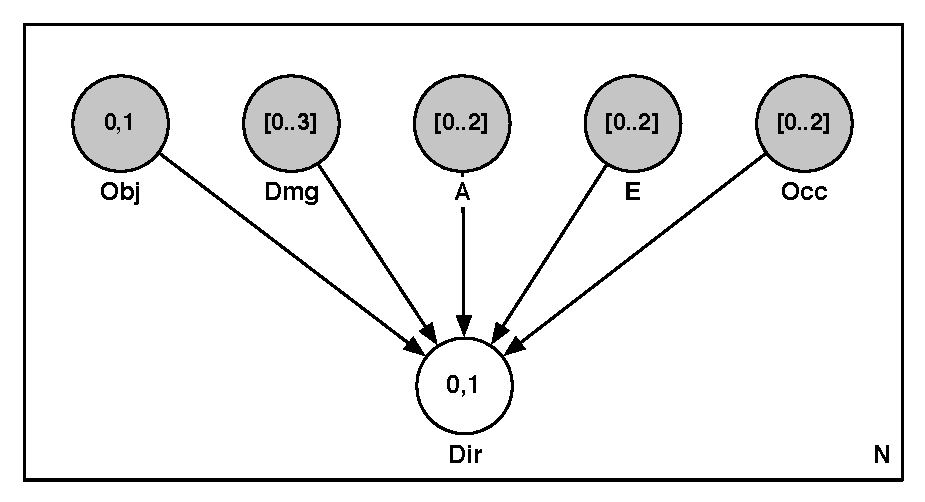
\includegraphics[width=8cm]{images/BayesianUnit_plate.pdf}
\caption{Plate diagram of a Bayesian unit with $N$ possible directions.}
\label{fig:BayesianUnit_plate}
\end{center}
\end{figure}

\section{Tactics}

\begin{table}[!h]
\begin{center}
\begin{tabular}{|llclccl|}
\hline
frame & player name & player id & order/action & X pos. & Y pos. & unit \\
\hline
$\vdots$ & $\vdots$ & $\vdots$ & $\vdots$ & $\vdots$ & $\vdots$ & $\vdots$ \\
6650 & L.Nazgul[pG] & 0 & Train & & & Probe\\
6720 & SaFT.eSu & 1 & Train & & & Probe\\
6830 & L.Nazgul[pG] & 0 & Train & & & Probe\\
7000 & SaFT.eSu & 1 & Train & & & Probe\\
7150 & L.Nazgul[pG] & 0 & Build & 39 & 108 & Forge\\
7245 & L.Nazgul[pG] & 0 & Build & 36 & 108 & Citadel of Adun\\
7340 & L.Nazgul[pG] & 0 & Train & & & Probe\\
7405 & SaFT.eSu & 1 & Train & & & Probe\\
7415 & L.Nazgul[pG] & 0 & Train & & & Probe\\
7480 & SaFT.eSu & 1 & Train & & & Shuttle\\
7510 & SaFT.eSu & 1 & Build & 26 & 24 & Robotics Support Bay\\
$\vdots$ & $\vdots$ & $\vdots$ & $\vdots$ & $\vdots$ & $\vdots$ & $\vdots$ \\
\hline
\end{tabular}
\caption{Example of what is in a replay (in human readable format), lines with non-empty positions are constructions of buildings. Several other action types are not represented (current selection, move/attack orders...)}
\label{tab:replay_example}
\end{center}
\end{table}

\begin{figure}[!h]
\begin{center}
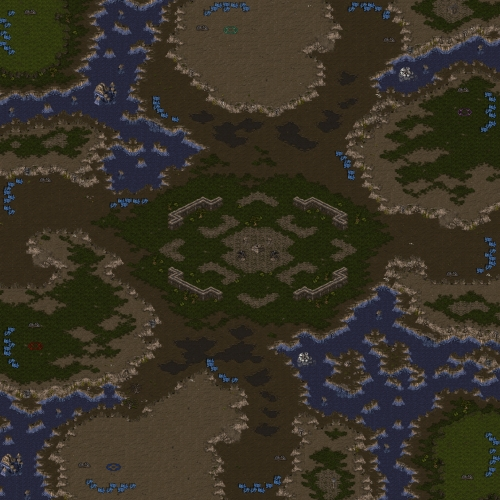
\includegraphics[width=11cm]{images/ICCup_lost_temple_24.jpg}
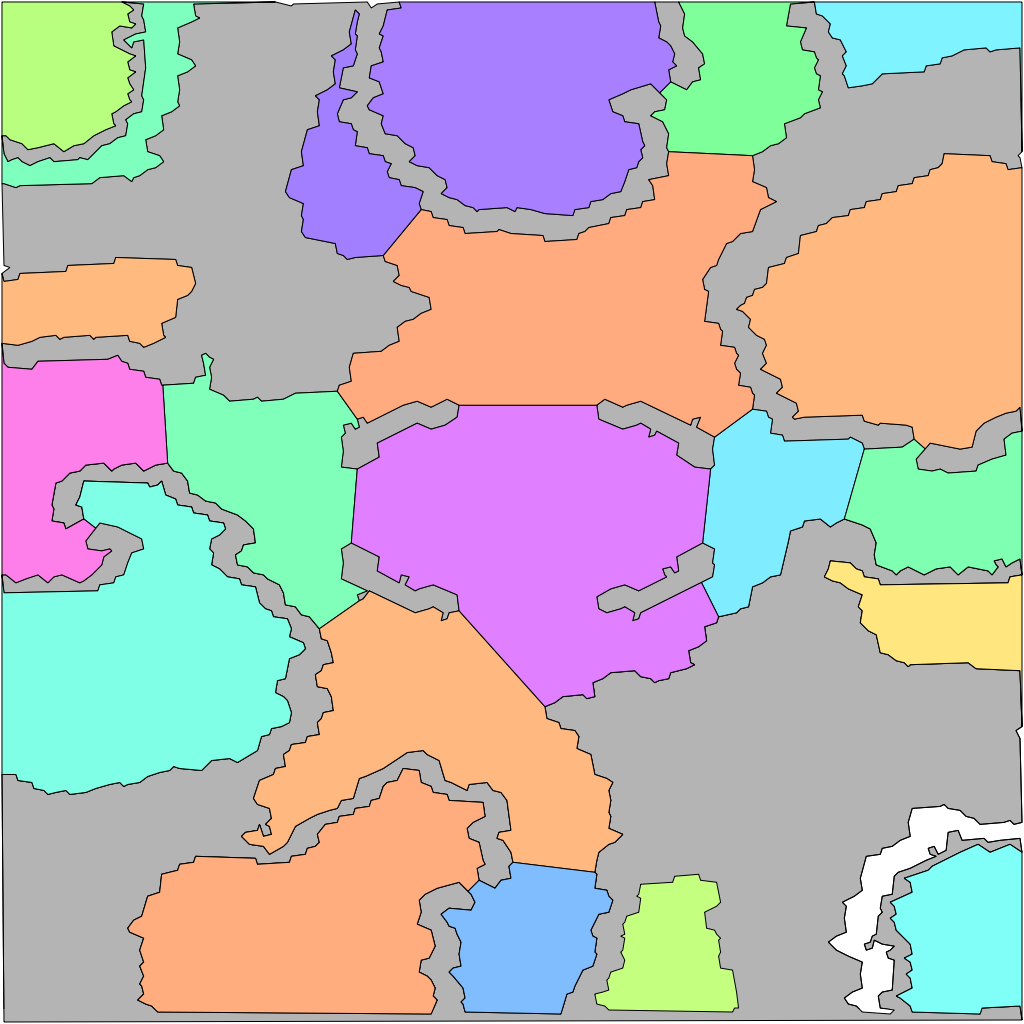
\includegraphics[width=11cm]{images/iccup_lost_temple_24scx-analyzed.png}
\caption{Top: StarCraft's Lost Temple map (one of the most famous maps with Python). We can see features like cliffs, ramps, walls, waters and resources (minerals and gas). Bottom: output of \glos{BWTA} with the \textit{regions} slicing. We can see regions with one or several chokes, but also isolated regions as gray is non walkable terrain (crossable by flying units only).}
\thispagestyle{empty}
\label{fig:BWTA}
\end{center}
\end{figure}

\begin{figure}[!h]
\begin{verbatim}
[Replay Start]
RepPath: $(PATH/TO/REP)
MapName: $MAPNAME
NumStartPositions: $N
The following players are in this replay:
<list of 
$PLAYER_ID, $PLAYER_NAME, $START_LOC
separated by newlines>
Begin replay data:
<list of
$FRAME_NUMBER,$PLAYER_ID,$ACTION,[$ACTION_DEP_ARGS]
separated by newlines>
[EndGame]
\end{verbatim}
\caption{Template of an RGD (replay general data) file from the dataset (see section~\ref{sec:dataset})}
\label{fig:rgdfile}
\end{figure}

\begin{figure}[!h]
\begin{verbatim}
<list of
$FRAME,$UNIT_ID,$ORDER,TargetOrPosition,$POS_X,$POS_Y
separated by newlines>
\end{verbatim}
\caption{Template of an ROD (replay order data) file from the dataset (see section~\ref{sec:dataset})}
\label{fig:rodfile}
\end{figure}

\begin{figure}[!h]
\begin{verbatim}
Regions,$REGIONS_IDS_COMMA_SEPARATED
$REGION_ID, $DIST, $DIST, ...
$REGION_ID, $DIST, $DIST, ...
.
.
.
ChokeDepReg,$REGIONS_IDS_COMMA_SEPARATED
$REGION_ID, $DIST, $DIST, ...
$REGION_ID, $DIST, $DIST, ...
.
.
.
[Replay Start]
<list of
$FRAME,$UNIT_ID,$POS_X,$POS_Y
$FRAME,$UNIT_ID,Reg,$REGION_ID
$FRAME,$UNIT_ID,CDR,$CDR_ID
separated by newlines>
\end{verbatim}
\caption{Template of an RLD (replay location data) file from the dataset (see section~\ref{sec:dataset})}
\label{fig:rldfile}
\end{figure}

\subsection{Decision-making: soft evidences and coherence variables}
\label{appdx:softevidences}

Here we will present the full tactical model for decision making, with soft evidences of variables we know only partially (variables we have only the distribution).

\subsubsection{Variables}
In the tactical model (section~\ref{sec:tacticalmodel}), for some variables, we take uncertainty into account with ``soft evidences'': for instance for a region in which no player has a base, we have a soft evidence that it belongs more probably to the player established closer. In this case, for a given region, we introduce the soft evidence variable(s) $B'$ and the \textit{coherence variable} $\lambda_B$ and impose $\PP(\lambda_B=1|B,B')=1.0\ iff\ B=B'$, else $\PP(\lambda_B=1|B,B')=0.0$; while $\PP(\lambda_B|B,B')\PP(B')$ is a new factor in the joint distribution. This allows to sum over $\PP(B')$ distribution (soft evidence). We do that for all the variables which will not be directly observed in decision-making.

\subsubsection{Decomposition}
%The joint distribution of our model contains soft evidence variables for all input family variables ($E,T,TA,B,GD,AD,ID,HP$) to be as general as possible, \textit{i.e.} to be able to cope with all possible uncertainty (from incomplete information) that may come up in a game. \textbf{To avoid being too verbose}, we explain the decomposition only with the soft evidence for the family of variables $B$, the principle holds for all other soft evidences. \textbf{We will enunciate the full model in the Bayesian program.} 
The joint distribution of our model contains soft evidence variables for all input family variables ($E,T,B,GD,AD,ID$) as we cannot know for sure the economical values of the opponent's regions under the \glos{fogofwar} ($E$), nor can we know exactly the tactical value ($T$) for them, nor the possession of the regions ($B$), nor the exact defensive scores ($GD,AD,ID$). Under this form, it deals with all possible uncertainty (from incomplete information) that may come up in a game. 
For the $n$ considered regions, we have:
%%% \begin{eqnarray}
%%%     & & \PP(A_{1:n}, E_{1:n}, T_{1:n}, TA_{1:n}, B_{1:n}, B'_{1:n}, \lambda_{B,1:n}, \\
%%% & & H_{1:n}, GD_{1:n}, AD_{1:n}, ID_{1:n}, HP, TT) \\
%%%     & = & \prod_{i=1}^n \left[\PP(A_i)\PP(E_i,T_i,TA_i,B_i|A_i) \label{eqn:tacticsdecomposition}\right.\\
%%% & & \PP(\lambda_{B,i} | B_{1:n},B'_{1:n})\PP(B'_{1:n}) \\
%%% & & \left. \PP(AD_i,GD_i,ID_i|H_i)\PP(H_i|HP)\right]\PP(HP|TT)\PP(TT)
%%% \end{eqnarray}
\begin{eqnarray}
    & & \PP(A_{1:n}, E_{1:n}, T_{1:n}, TA_{1:n}, B_{1:n}, 
B'_{1:n}, \lambda_{B,1:n}, T'_{1:n}, \lambda_{T,1:n}, \\
& & E'_{1:n}, \lambda_{E,1:n},
ID'_{1:n}, \lambda_{ID,1:n},
GD'_{1:n}, \lambda_{GD,1:n},
AD'_{1:n}, \lambda_{AD,1:n},\\
& & H_{1:n}, GD_{1:n}, AD_{1:n}, ID_{1:n}, HP, TT) \\
    & = & \prod_{i=1}^n \left[\PP(A_i)\PP(E_i,T_i,TA_i,B_i|A_i) \right.\\
& & \PP(\lambda_{B,i} | B_{1:n},B'_{1:n})\PP(B'_{1:n}) 
\PP(\lambda_{T,i} | T_{1:n},T'_{1:n})\PP(T'_{1:n}) \\
& & \PP(\lambda_{E,i} | E_{1:n},E'_{1:n})\PP(E'_{1:n}) 
\PP(\lambda_{ID,i} | ID_{1:n},ID'_{1:n})\PP(ID'_{1:n}) \\
& & \PP(\lambda_{GD,i} | GD_{1:n},GD'_{1:n})\PP(GD'_{1:n})
\PP(\lambda_{AD,i} | AD_{1:n},AD'_{1:n})\PP(AD'_{1:n}) \\
& & \left. \PP(AD_i,GD_i,ID_i|H_i)\PP(H_i|HP)\right]\PP(HP|TT)\PP(TT)
\end{eqnarray}

The full plate diagram of this model is shown in Figure~\ref{fig:SpecialTacticsFull_plate}.
\begin{figure}[h]
\begin{center}
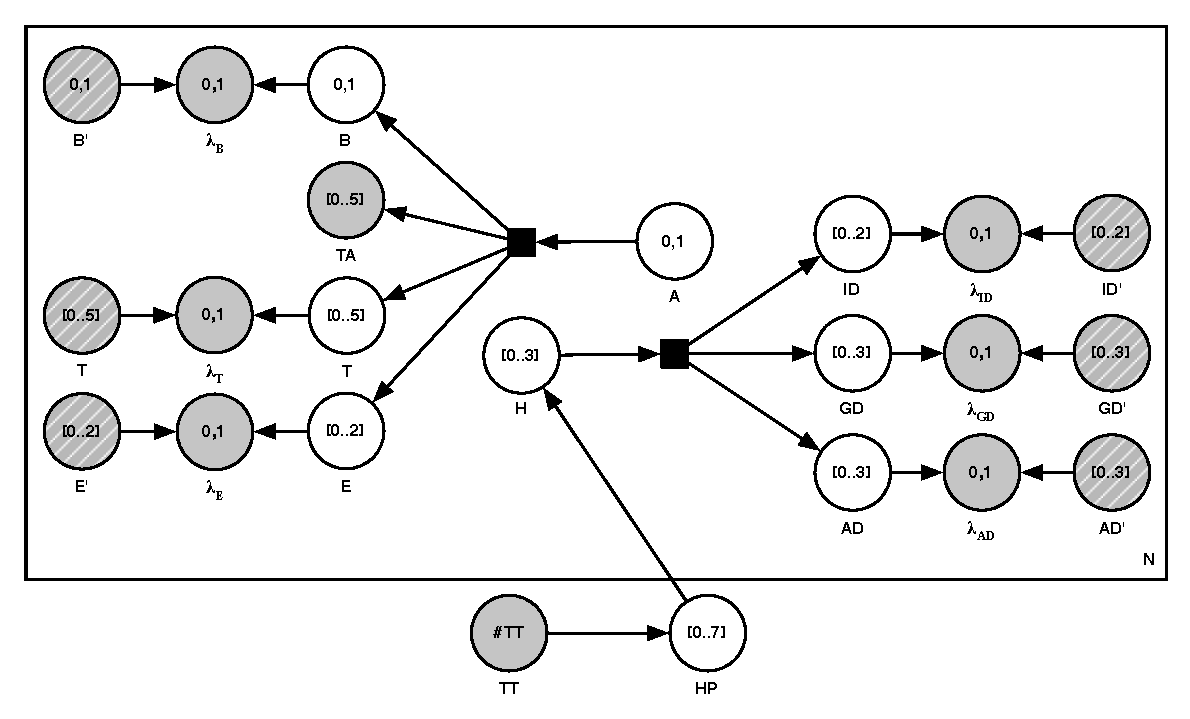
\includegraphics[width=15cm]{images/SpecialTacticsFull_plate.pdf}
\caption{Plate diagram (factor graph notation) of the Bayesian tactical model in decision-making mode. Hatched nodes are nodes on which we only have a distribution. We know $TA$ (our tactical scores as we are the attacker) and $TT$ (our \glos{techtree}).}
\label{fig:SpecialTacticsFull_plate}
\end{center}
\end{figure}

\subsubsection{Forms}

To the previous forms (section~\ref{sec:tacticaldecomposition}), we add for all variables which were doubles ($X$ with $X'$):
\begin{eqnarray*}
\begin{cases}
\PP(\lambda_{X}|X,X') = 1.0\ \mathrm{iff}\ X=X'\\
\PP(\lambda_{X}|X,X') = 0.0\ \mathrm{else}
\end{cases}
\end{eqnarray*}
%%% \begin{itemize}
%%% \item $\PP(\lambda_{B}|B,B') = 1.0\ iff\ B=B'$ is just a coherence constraint.
%%% \end{itemize}
\subsubsection{Identification}
The identification and learning does not change, c.f. section~\ref{sec:tacticalidentification}.

\subsubsection{Questions}
\begin{footnotesize}
\begin{eqnarray*}
&  & \forall i \in regions\ \PP(A_i|ta_i,\lambda_{B,i}=1,\lambda_{T,i}=1,\lambda_{E,i}=1)\\
& \propto & \int_{B_i,B_i'} \int_{T_i,T_i'} \int_{E_i,E_i'} \PP(E_i,T_i,ta_i,B_i|A_i)\PP(A_i)\PP(B_i')\PP(T_i')\PP(E_i')\\
& & \forall i \in regions\ \PP(H_i|tt,\lambda_{ID,i}=1,\lambda_{GD,i}=1,\lambda_{AD,i}=1)\\
& \propto & \int_{ID_i,ID_i'}\int_{GD_i,GD_i'}\int_{AD_i,AD_i'}\sum_{HP}\PP(AD_i,GD_i,ID_i|H_i)\PP(H_i|HP)\PP(HP|tt)\PP(ID_i')\PP(AD_i')\PP(GD_i')
\end{eqnarray*}
\end{footnotesize}

\subsubsection{Bayesian program}
The Bayesian program of the model is as follows: %(\ref{bp:BayesianTacticianFull}):
%\begin{figure}[!h]
\begin{footnotesize}
\begin{eqnarray*}
\begin{sideways}\parbox{35mm}{\hspace{-1.3cm}Bayesian program}\end{sideways}
\begin{cases}
\begin{sideways}\parbox{15mm}{\hspace{-0.8cm}Description}\end{sideways}
    \begin{cases}
    
\begin{sideways}\parbox{35mm}{\hspace{-1.1cm}Specification ($\pi$)}\end{sideways}
        \begin{cases}

        Variables\\

A_{1:n}, E_{1:n}, T_{1:n}, TA_{1:n}, B_{1:n}, 
B'_{1:n}, \lambda_{B,1:n}, T'_{1:n}, \lambda_{T,1:n},
E'_{1:n}, \lambda_{E,1:n},\\
ID'_{1:n}, \lambda_{ID,1:n},
GD'_{1:n}, \lambda_{GD,1:n},
AD'_{1:n}, \lambda_{AD,1:n},
H_{1:n}, GD_{1:n}, AD_{1:n}, ID_{1:n}, HP, TT\\

        Decomposition\\

\PP(A_{1:n}, E_{1:n}, T_{1:n}, TA_{1:n}, B_{1:n}, 
B'_{1:n}, \lambda_{B,1:n}, T'_{1:n}, \lambda_{T,1:n},
 E'_{1:n}, \lambda_{E,1:n},\\
ID'_{1:n}, \lambda_{ID,1:n},
GD'_{1:n}, \lambda_{GD,1:n},
AD'_{1:n}, \lambda_{AD,1:n},
H_{1:n}, GD_{1:n}, AD_{1:n}, ID_{1:n}, HP, TT) \\
     = \prod_{i=1}^n \left[\PP(A_i)\PP(E_i,T_i,TA_i,B_i|A_i) \right.
\PP(\lambda_{B,i} | B_{1:n},B'_{1:n})\PP(B'_{1:n}) 
\PP(\lambda_{T,i} | T_{1:n},T'_{1:n})\PP(T'_{1:n}) \\
\PP(\lambda_{E,i} | E_{1:n},E'_{1:n})\PP(E'_{1:n})
\PP(\lambda_{ID,i} | ID_{1:n},ID'_{1:n})\PP(ID'_{1:n}) 
\PP(\lambda_{GD,i} | GD_{1:n},GD'_{1:n})\PP(GD'_{1:n})\\
\PP(\lambda_{AD,i} | AD_{1:n},AD'_{1:n})\PP(AD'_{1:n})
\left. \PP(AD_i,GD_i,ID_i|H_i)\PP(H_i|HP)\right]\PP(HP|TT)\PP(TT)\\

        Forms\\

\PP(A_r)\ \mathrm{prior\ on\ attack\ in\ region}\ i\\
\PP(E,T,TA,B|A)\ \mathrm{covariance/probability\ table}\\ 
\PP(\lambda_{X}|X,X') = 1.0\ \mathrm{iff}\ X=X',\ \mathrm{else}\ \PP(\lambda_{X}|X,X') = 0.0\ (Dirac)\\ 
\PP(AD,GD,ID|H)\ \mathrm{covariance/probability\ table}\\
\PP(H|HP) = Categorical(4,HP)\\
\PP(HP=hp|TT) = 1.0\ iff\ TT\rightarrow hp,\ else\ \PP(HP|TT)=0.0\\
\PP(TT)\ \mathrm{comes\ from\ a\ strategic\ model}\\
        \end{cases}\\

    Identification\ (using\ \delta)\\
\PP(A_r=true)= \frac{n_{battles}}{n_{battles}+n_{not\ battles}} = \frac{\mu_{battles/game}}{\mu_{regions/map}}\ \mathrm{(probability\ to\ attack\ a\ region)}\\
\mathrm{it\ could\ be\ learned\ online\ (preference\ of\ the\ opponent):}\\
\PP(A_r=true) = \frac{1 + n_{battles}(r)}{2 + \sum_{i \in regions}n_{battles}(i)}\ \mathrm{(online\ for\ each\ game)}\\
\PP(E=e,T=t,TA=ta,B=b|A=True) = \frac{1+n_{battles}(e,t,ta,b)}{\abs{E} \times \abs{T} \times \abs{TA} \times \abs{B} + \sum_{E,T,TA,B} n_{battles}(E,T,TA,B)} \\
\PP(AD=ad,GD=gd,ID=id|H=h) = \frac{1+n_{battles}(ad,gd,id,h)}{\abs{AD} \times \abs{GD} \times \abs{ID} + \sum_{AD,GD,ID} n_{battles}(AD,GD,ID,h)} \\
\PP(H=h|HP=hp) = \frac{1 + n_{battles}(h,hp)}{\abs{H} + \sum_{H} n_{battles}(H,hp)}\\
    \end{cases}\\
Questions\\
\mathrm{decision-making}\\
\forall i \in regions \PP(A_i|ta_i,\lambda_{B,i}=1,\lambda_{T,i}=1,\lambda_{E,i}=1)\\
\forall i \in regions \PP(H_i|tt,\lambda_{ID,i}=1,\lambda_{GD,i}=1,\lambda_{AD,i}=1) \\
\end{cases}
\label{bp:BayesianTacticianFull}
\end{eqnarray*}
\end{footnotesize}
%\end{figure}




\clearpage
\section{Strategy}

%%% \subsection{Openings and tech tree prediction dataset}
%%% \label{appdx:datasets}


%%% \begin{figure}[htp]
%%% \centerline{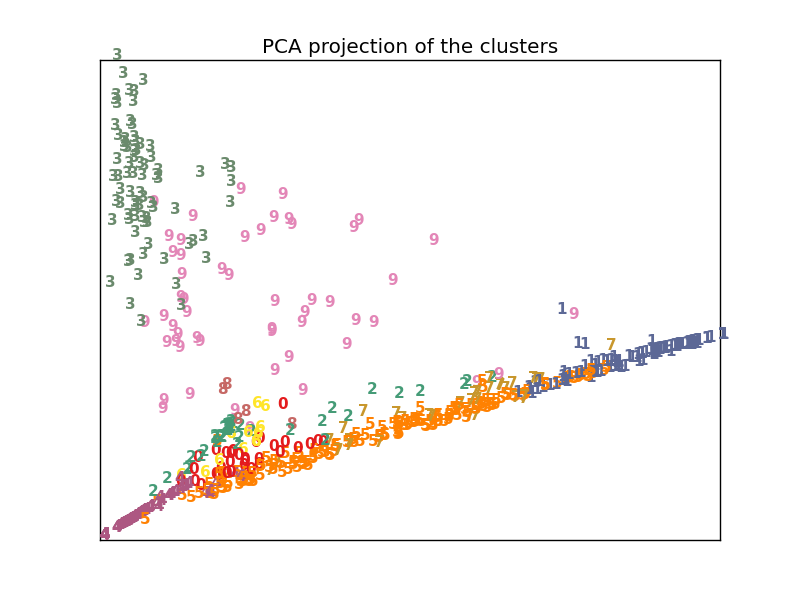
\includegraphics[width=0.98\columnwidth]{images/GMM_PCA_Z.png}}
%%% \centerline{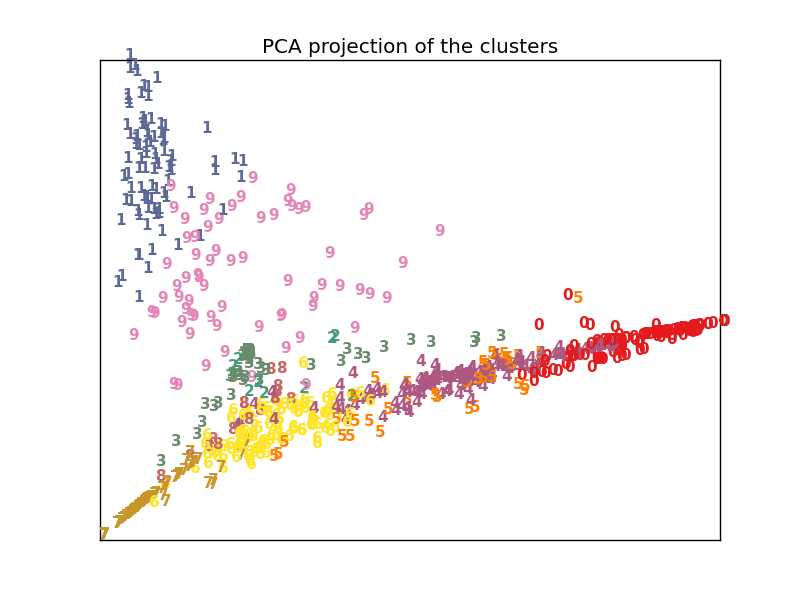
\includegraphics[width=0.98\columnwidth]{images/GMM_PCA_Z2.png}}
%%% \caption{GMM PCA Z XXXXXXX}
%%% \label{gmmpcaz}
%%% \end{figure}
%%% 
%%% \begin{figure}[htp]
%%% \centerline{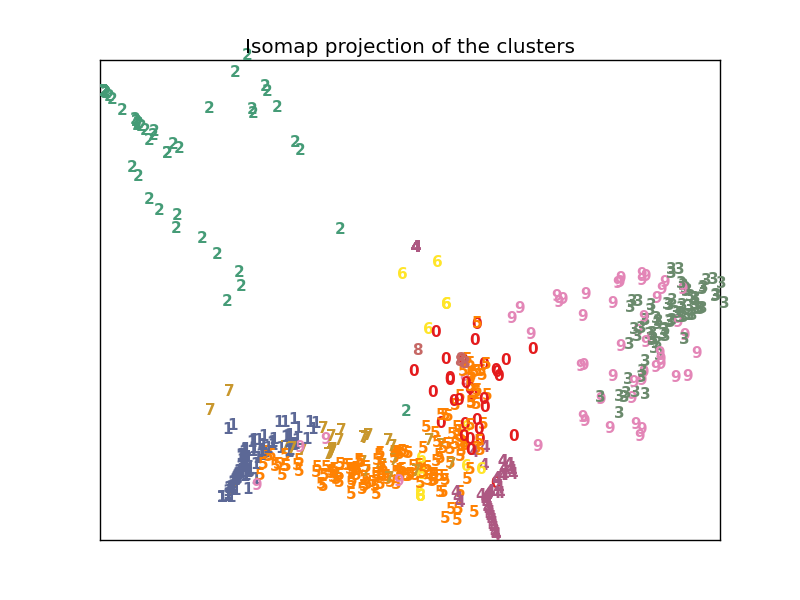
\includegraphics[width=0.98\columnwidth]{images/GMM_ISO_Z.png}}
%%% \centerline{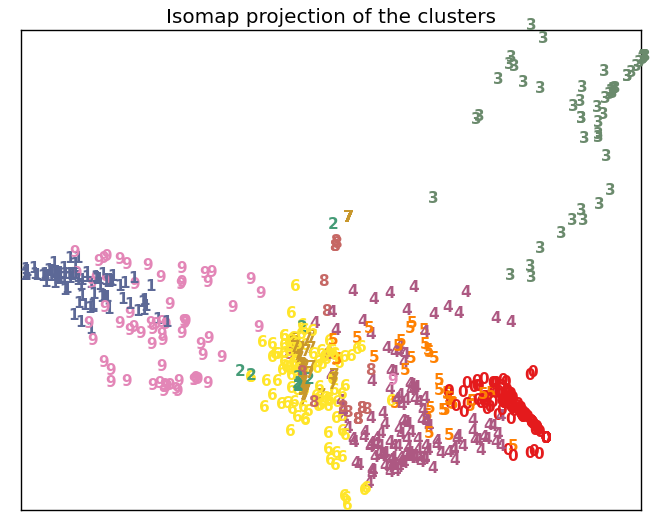
\includegraphics[width=0.98\columnwidth]{images/GMM_ISO_Z2.png}}
%%% \caption{GMM ISO Z XXXXX}
%%% \label{gmmisoz}
%%% \end{figure}
%%% 
%%% \begin{figure}[htp]
%%% \centerline{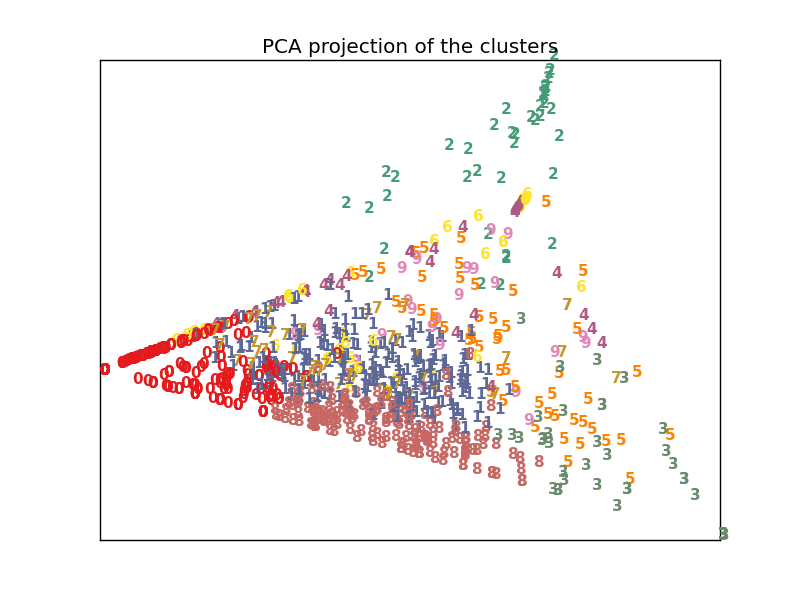
\includegraphics[width=0.98\columnwidth]{images/GMM_PCA_P.png}}
%%% \centerline{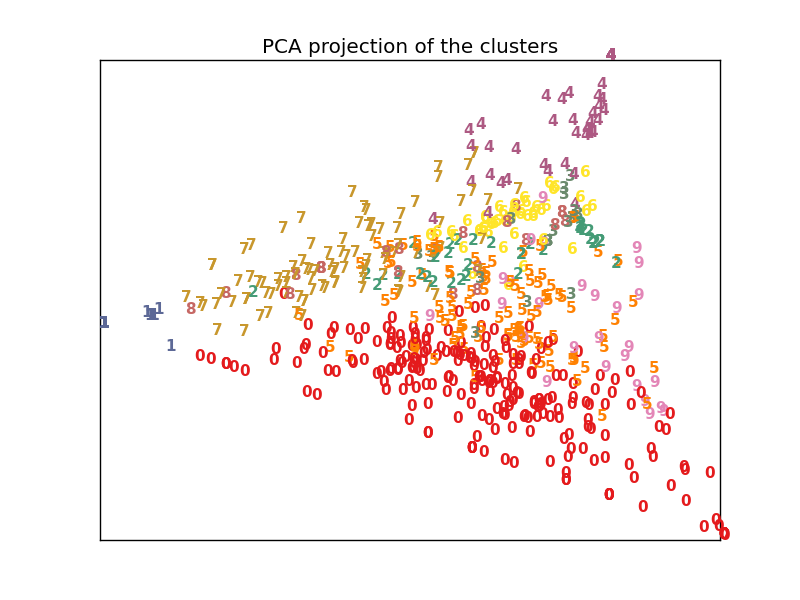
\includegraphics[width=0.98\columnwidth]{images/GMM_PCA_P2.png}}
%%% \caption{GMM PCA P XXXXX}
%%% \label{gmmpcap}
%%% \end{figure}
%%% 
%%% \begin{figure}[htp]
%%% \centerline{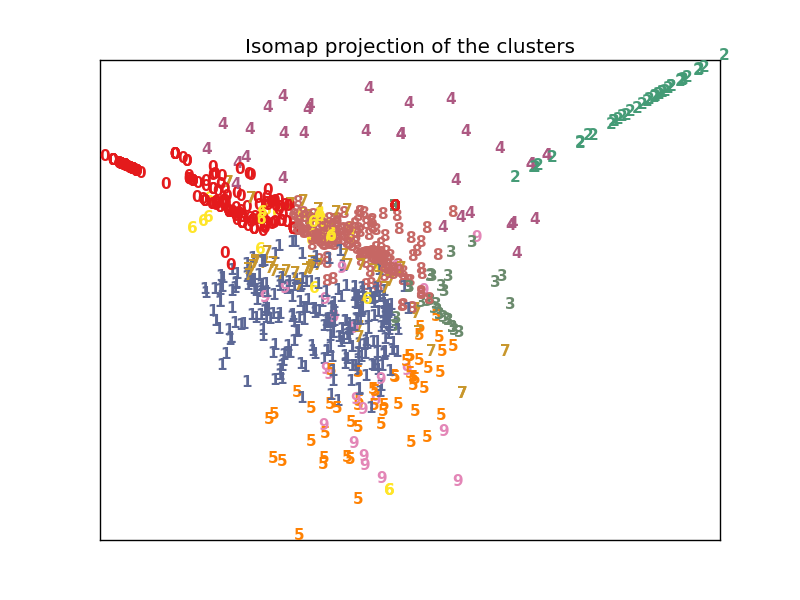
\includegraphics[width=0.98\columnwidth]{images/GMM_ISO_P.png}}
%%% \centerline{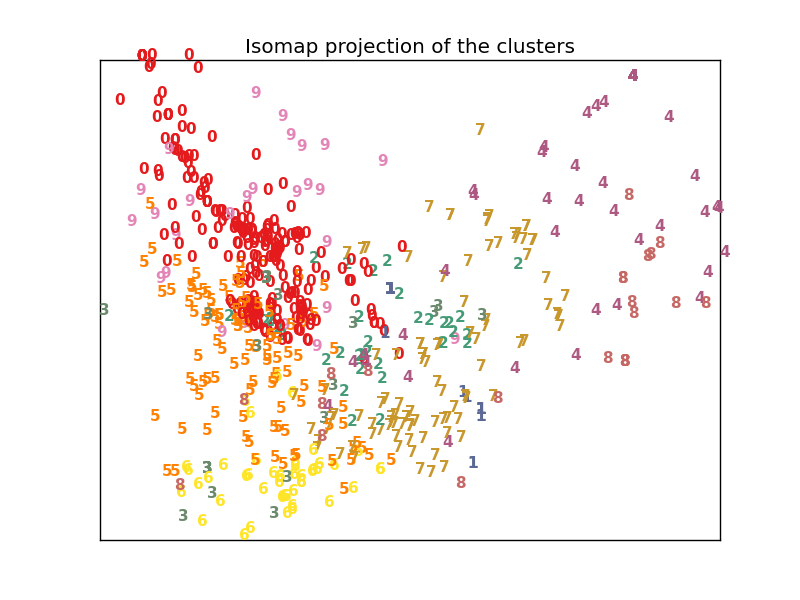
\includegraphics[width=0.98\columnwidth]{images/GMM_ISO_P2.png}}
%%% \caption{GMM ISO P XXXXX}
%%% \label{gmmisop}
%%% \end{figure}
%%% 


\section{\textsc{BroodwarBotQ}}
\begin{algorithm}
\caption{Flow algorithm making sure there are no convex closures}
\label{alg:flood}
\begin{algorithmic}
\Function{init}{$region$}
    %\State $\{Flow_{i,j} \leftarrow -1 | Flow_{i,j} \in region\}$
    %\State $\{Dir_{i,j} \leftarrow (0,0) | Dir_{i,j} \in region\}$
    \State $\{dir_{i,j} \leftarrow list() | (i,j) \in region\}$
    \State $updated \leftarrow \{(i,j) | (i,j) \in entrance(region)\}$
    %\State $\{Flow_{i,j} \leftarrow 1 | (i,j) \in Updated\}$
    \State $\{dir_{i,j} \leftarrow dir\_towards(region) | (i,j) \in updated\}$
    %\While{$(\exists Flow_{i,j} == -1) \ \mathrm{or}\ (\exists Dir_{i,j} == (0,0))$}
    \While{$\exists dir_{i,j} == list()$}
        \State $(sources,new\_updated) \leftarrow neighbours\_couples(updated)$
        \ForAll{$((x,y),(i,j)) \in (sources,new\_updated)$}
            %\If{$(i-x,j-y) \neq Dir_{x,y}$}
            \If{$(x-i,y-j) \notin dir_{x,y}$}
                \State $dir_{i,j}.append((i-x, j-y))$
            %    \State $Flow_{i,j} += 1$
            \EndIf
        \EndFor
        \State $updated \leftarrow new\_updated$
    \EndWhile
\EndFunction

\Function{build}{$i,j$}
\State $refill \leftarrow list()$
\ForAll{$(x,y) \in neighbours(i,j)$} \Comment{cut the flow arround}
    \State $dir_{x,y}.remove((x-i, y-j))$
    \If{$dir_{x,y}.empty()$}
        \State $refill.append((x,y))$
        \State $build(x,y)$ \Comment{Recursively cut the flow}
    \EndIf
\EndFor
\While{$\neg fixed\_point$} \Comment{refill as in the initialization...}
    \State $current \leftarrow dir$
    \ForAll{$(x,y) \in refill$}
        %\Comment{neighbour with a non empty flow}
        \If{$\exists (i,j) \in neighbours(x,y)$ such that $current_{i,j} \neq list() $}             
        \Comment{non empty flow}
            \State $dir_{x,y}.append((x-i, y-j))$
        \EndIf
    \EndFor
\EndWhile
\EndFunction


\Function{is\_isolated?}{$i,j$}
    \If{$dir_{i,j}.empty()$}
        \State \Return True
    \Else
        \State \Return False
    \EndIf
\EndFunction
\end{algorithmic}
\end{algorithm}

\begin{figure}[!h]
\begin{center}
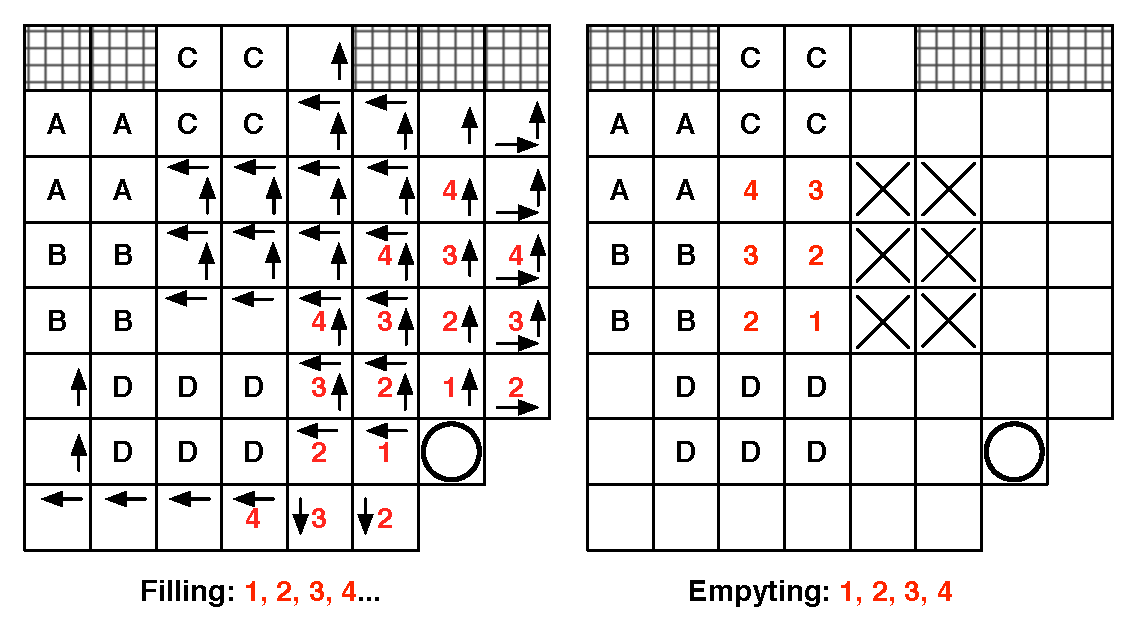
\includegraphics[width=13cm]{images/flow_buildings_placer.pdf}
\caption{Example of the algorithm~\ref{alg:flood} in a case in which there are buildings A, B, C, D and building in the new cross spots would close the paths to the interior and trap units. Left: flood filling of the region with the source at the choke (bottom right). The arrows show the $dir$ vectors for each tile. Right: recursive calls to \texttt{build} which drain the interior zone. Refilling will not be able to refill the middle.}
\label{fig:buildingsplacer}
\end{center}
\end{figure}

%%% \begin{algorithm}
%%% \caption{Production/Construction Planning}
%%% \label{alg:planning}
%%% \begin{algorithmic}
%%% \Function{init}{}
%%% \EndFunction
%%% \end{algorithmic}
%%% \end{algorithm}


\begin{figure}
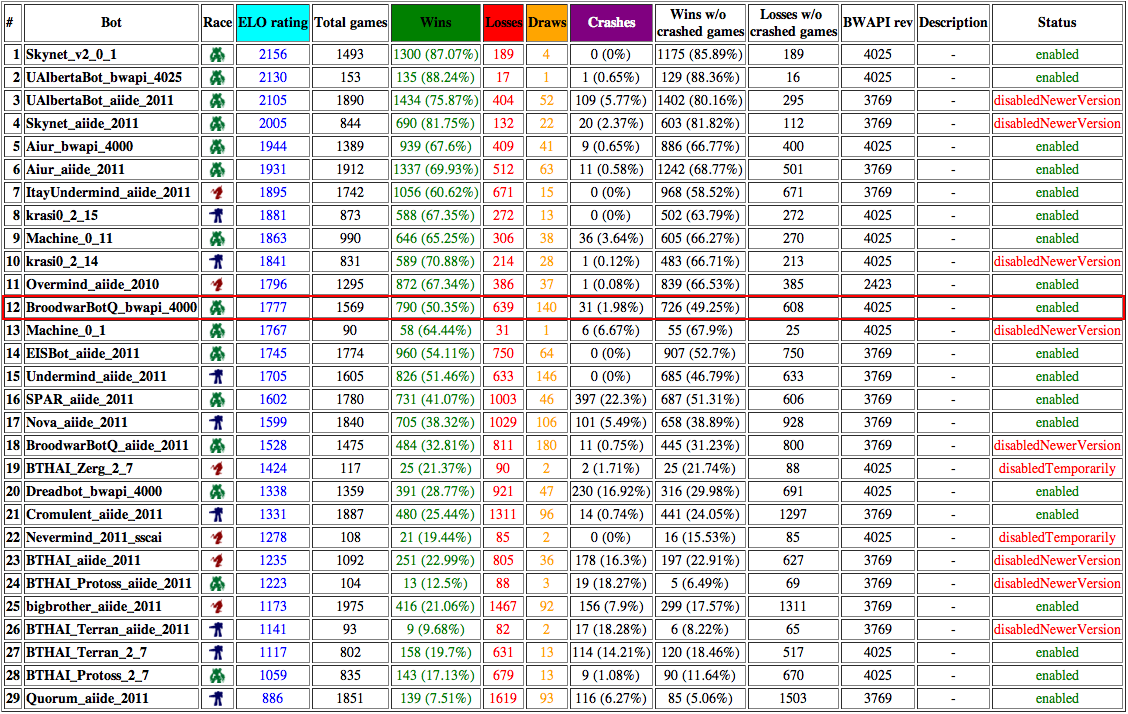
\includegraphics[width=1.0\columnwidth]{images/ladder_2012-02-12.png}
\caption{Bots ladder on February 12th, 2012. With \textsc{BroodwarBotQ} using a Bayesian model for opponent's strategy prediction as well as for \glos{micro}.}
\label{fig:ladderbots}
\end{figure}
